\documentclass{llncs}
\usepackage{times}
\usepackage[portuguese]{babel}
\usepackage[utf8]{inputenc}
\usepackage[T1]{fontenc}

% Comentar para not MAC Users
% \usepackage[applemac]{inputenc}

\usepackage{a4}
%\usepackage[margin=3cm,nohead]{geometry}
\usepackage{epstopdf}
\usepackage{graphicx}
\usepackage{fancyvrb}
\usepackage{amsmath}
\usepackage{float}
\usepackage{indentfirst}
%\renewcommand{\baselinestretch}{1.5}

\begin{document}

\title{Relatório TP2}
\titlerunning{Relatório TP2}
\author{Carlos Silva, João Coelho e Miguel Silva}
\authorrunning{Carlos Silva, João Coelho e Miguel Silva}

\institute{
Universidade do Minho, Departamento de Informática, 4710-057 Braga, Portugal\\
e-mail: \{a75107,a74859,a74601\}@alunos.uminho.pt
}

%\para não aparecer data
\date{}
\bibliographystyle{splncs}

\maketitle

\begin{abstract}
Este trabalho expõe uma situação de necessidade de escolha perante vários servidores Web, procurando não só propor uma solução para situações semelhantes, como também expor a importância deste tipo de seleção, de modo a aumentar a eficácia da resposta aos pedidos. Desde a arquitetura à implementação e posteriores testes, neste documento apresenta-se o relatório de todo o processo de desenvolvimento do tema.
\end{abstract}

\newpage

\section{Introdução}

\subsection{Contextualização}

Em muitos serviços Web, um único servidor não é suficiente para dar vazão aos pedidos dos clientes. Nesses casos, é necessário ter uma pool de N servidores de back-end, capazes de dar resposta aos pedidos. Ainda assim, o serviço terá um único ponto de entrada, comum a todos os
clientes, que se trata de um servidor de front-end, com nome e endereço IP únicos e bem conhecidos. A tarefa deste servidor, habitualmente designado por \textit{Reverse Proxy}, é atender as conexões dos clientes e desviá-las para um dos servidores de back-end disponíveis.\par
A escolha do servidor pode ser cega, baseada por exemplo num algoritmo de Round-Robin, que faz uma distribuição equitativa das conexões pelos N servidores de back-end, mas será esta a melhor solução?

\subsection{Exposição do problema}

O principal objetivo deste trabalho é desenhar e implementar um serviço simples de proxy reverso TCP, em que a escolha do servidor a usar se
faz com base em parâmetros dinâmicos, como por exemplo o RTT, as perdas e número de conexões TCP do servidor. Para tal, é necessário haver monitorização dos dados do estado do servidor e da rede, redirecionando em função de uma métrica dinâmica bem definida. Pretende-se desenhar e implementar um protótipo simples desta abordagem, separando-a em dois momentos: numa primeira fase temos um protocolo sobre UDP, para criar e manter atualizada uma tabela com dados recolhidos por agentes de monitorização; depois, numa segunda fase, pretende-se implementar um servidor proxy TCP genérico, que fique à escuta na porta 80 e redirecione, automaticamente, cada conexão TCP que recebe para a porta 80 de um dos servidores de back-end disponíveis (o que aparente estar em melhores condições para o fazer).

\begin{figure}[H]
\centering
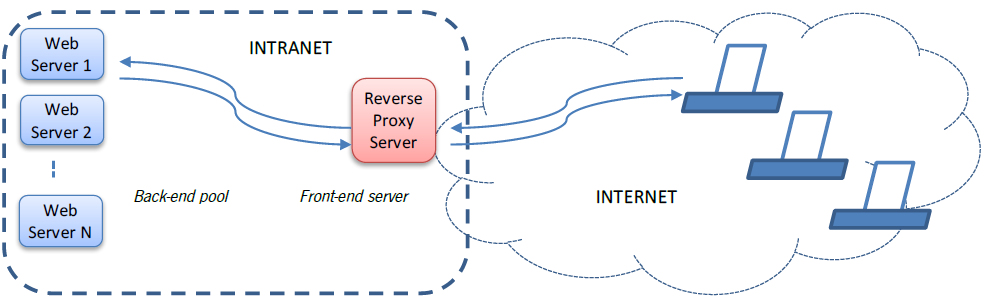
\includegraphics[width=150mm, scale=0.5]{imagem_enunciado.PNG}
\caption{\label{fig:change}Esquematização da arquitetura do problema.}
\end{figure}

\newpage

\section{Arquitetura da solução implementada(em ambiente de teste)}
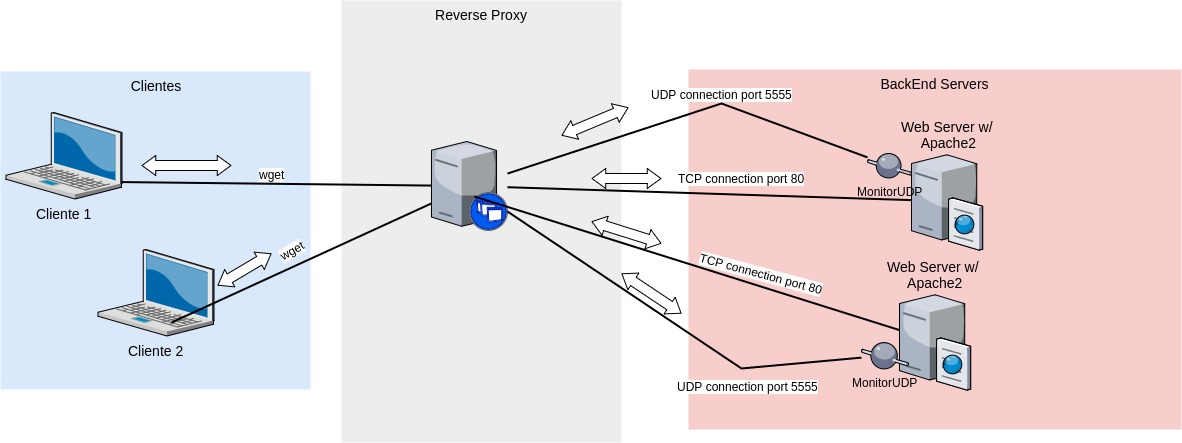
\includegraphics[width=160mm, scale=1]{imagemArq.jpg}

\newpage

\section{Especificação do protocolo de monitorização}

\begin{itemize}
	\setlength\itemsep{1em}
\item \textbf{Primitivas de comunicação:} Sockets UDP.
\item \textbf{Formato do PDU:} constituído pelo número do ACK do próximo pacote, que o servidor pretende receber, e pelo timestamp que permitirá calcular o RTT. Sobre o ACK, importa referir que é utilizado no cálculo do taxa de perdas e de duplicados. Já sobre o timestamp, nota para o cuidado especial que se teve para que contabilizasse apenas o tempo de deslocamento de um pacote entre servidores. Aquando da receção de um pacote, o monitor marca o momento. A esse valor temporal subtrai o timestamp recebido, obtendo assim o tempo da deslocação até si. Depois, no momento em que se prepara para enviar a resposta ao pedido de probing, volta a calcular o tempo atual, subtraindo o valor do tempo da deslocação. Assim, ao receber a resposta, o \textit{Reverse Proxy} só tem de calcular o momento atual e subtrair o timestamp recebido na resposta, obtendo assim o RTT.
\item \textbf{Interações:} Os servidores \textit{back-end} disponíveis enviam \textit{hellos} de 5 em 5 segundos, com o \textit{Reverse Proxy} a responder aos mesmos com pedidos de \textit{probing}.
\end{itemize}

\newpage

\section{Implementação}

\begin{itemize}
	\setlength\itemsep{1em}
	\setlength{\parindent}{1cm}
\item \textbf{Monitor UDP:} Cada \textit{back-end} terá associado a si um monitor implementado via UDP, que monitoriza o estado da ligação com o \textit{Reverse Proxy}. O monitor envia \textit{hellos} de 5 em 5 segundos para o \textit{Reverse Proxy} e responde ao pedido de \textit{probing} por parte do servidor. Para o tratamento do envio dos \textit{hellos}, foi implementada uma thread que se dedica somente a isso.\par
	A thread principal do monitor é a responsável por responder aos pedidos que o \textit{back-end} faz quando deseja atualizar a entrada da tabela que correponde ao presente monitor. Assim, sempre que é recebido um pacote no monitor vindo do \textit{Reverse Proxy}, é recebido o número de sequência desse pacote, sendo a esse número adicionada uma unidade que advém de agora o monitor esperar pelo próximo pacote. É, portanto, enviado no PDU o número de sequência que corresponde ao próximo pacote que o monitor está à espera. É também calculado e enviado no PDU um \textit{timestamp}, já esclarecido na secção acima.\par
	Esta comunicação por UDP foi implementada com o auxílio da API de \textit{DatagramPackets}.
	
	\item \textbf{\textit{Reverse Proxy}:} O \textit{Reverse Proxy} tem a função de selecionar um servidor \textit{back-end} para dar resposta a pedidos de clientes de forma mais rápida e eficiente.\par 
	Assim, é necessário enviar pedidos de \textit{probing} aos \textit{back-ends} que estão ligados, de forma a que a escolha do servidor seja a melhor possível. O envio e receção de \textit{probing} são assegurados por uma nova thread criada para o paralelismo dos processos. Estes pedidos são enviados logo que um \textit{hello} vindo de um monitor é recebido, ou seja, de 5 em 5 segundos também. O pedido enviado é tratado pelo monitor da forma referida no ponto anterior, e depois recebido novamente pelo \textit{Reverse Proxy}, que retira informação do PDU que lhe chega. Esta informação ajuda a atualizar a tabela com os dados dos monitores, como o RTT (\textit{round-trip-time}), número de pacotes duplicados e a \textit{loss rate} (percentagem de pacotes perdidos).\par 
	O RTT é calculado através do timestamp que traz consigo o PDU. Este timestamp já conta com o deslocamento incial \textit{Reverse Proxy} --> \textit{back-end}, sendo que quando recebido, agora é somente necessário subtrair o timestamp atual pelo que veio com o PDU. A cada pacote com a resposta/pedido de \textit{probing}, são incrementados o número de pacotes enviados e o número de pacotes recebidos. Este controlo de pacotes que são enviados e recebidos é usado para ser calculada a \textit{loss rate}. O número de pacotes duplicados são calculados com recurso aos ACKs que são enviados e recebidos. Quando é recebido mais do que um pacote com o mesmo ACK é incrementado o número de pacotes duplicados, para o monitor em questão. Toda esta informação é atualizada para a entrada da tabela, correspondente a cada monitor.\par
	O \textit{Reverse Proxy}, além de tratar de toda a monitorização dos \textit{back-ends} via UDP utilizando DatagramPackets, como se acabou de expôr, trata também da receção e encaminhamento de um pedido de um cliente para o melhor \textit{back-end} no momento, via TCP.\par
	Para a escolha do melhor \textit{back-end} para encaminhamento, é utilizado um score que é calculado utilizando informação presente na tabela deste. Assim, para o cálculo do score, o \textit{loss rate} é multiplicado por 100, o número de conexões TCP é multiplicado por 2 e o número de pacotes duplicados é dividido pelo número total de pacotes enviados e recebidos, de modo a que a \textit{loss rate} e o número de conexões TCP tenham mais significância e os duplicados não tenham tanto peso. O score é então a soma destes três parâmetros mais o RTT. A cada 5 segundos, o score é reiniciado.\par
	A receção do pedido do cliente, o encaminhamento do pedido do cliente para o melhor \textit{back-end} disponível e a receção da resposta do \textit{back-end} são tratados numa nova thread criada para este propósito. \par
	Finalmente, se um \textit{back-end} não mandar \textit{hellos} durante um período contíguo de 20 segundos, o \textit{Reverse Proxy} retira a entrada da tabela que é correspondente ao \textit{back-end} que não se mostra disponível. Esta funcionalidade é também tratada numa nova thread, criada para este mesmo propósito.
	
	
	

\end{itemize}
\newpage

\section{Testes e resultados}

Para cenário de teste foi utilizado Apache2 em cada um dos servidores \textit{back-end}(dois),
uma máquina a correr o \textit{Reverse Proxy} e ainda dois clientes a efetuar pedidos ao \textit{Reverse Proxy}. Os testes foram realizados na topologia core da unidade curricular, a máquina do \textit{Reverse Proxy} é o Servidor 1, as máquinas de \textit{back-end} são os portáteis 1 e 2 e, por último, os clientes que são o 1 e 2.\par
Deixou-se a topologia correr, durante alguns segundos, o \textit{Reverse Proxy} e os 2 servidores \textit{back-end} para que a tabela do \textit{Reverse Proxy} estabilizasse. Depois, efetuou-se o comando wget no Cliente 1 para o \textit{Reverse Proxy} obtendo o index.html do servidor \textit{back-end} com melhor score naquele instante. Verificou-se que o número de conexões TCP (na tabela) do servidor \textit{back-end}, naquele momento, aumentou para 1, então testou-se um wget de cada cliente e o número de conexões TCP do \textit{back-end} escolhido atualizou para 2. Como os pedidos dos clientes não foram efetuados exatamente ao mesmo tempo, também existiu a situação em que cada pedido foi atendido por um servidor \textit{back-end} diferente, ficando ambos com uma conexão TCP naquele momento.

\newpage

\section{Conclusões e trabalho futuro}

Tendo em conta que os resultados obtidos foram satisfatórios, considera-se que a solução implementada é plausível e de aceitável eficiência. Todavia, para uma maior fiabilidade dos resultados, seria necessário testar o programa fora da topologia CORE utilizada. Uma situação mais realista, com máquinas diferentes a correrem o programa, era recomendável. Isto permitiria, por exemplo, tornar mais rigorosa a contagem do número de conexões TCP, permitindo o uso de comandos como o netstat.\par
Para além do aprofundar dos testes, outra secção a explorar no futuro seria o algoritmo de seleção do servidor \textit{back-end}. Com mais alguma reflexão, inclusão de outras variáveis e, também, melhores testes, antecipa-se que os resultados seriam melhores. Porém, sublinhando, a solução implementada foi satisfatória a este nível.

\newpage
%UNCOMMENT para a bibliografia 
%% ficheirodebibliografia.bib
%\bibliography{ficheirodebibliografia}

%ou inserir directamente os v‡rios \bibitem 
\begin{thebibliography}{1}

\bibitem{Computer Networking}
Kurose, J., Ross K.: Computer Networking . A Top Down Approach Featuring the Internet, 6ª edição (2012)

%Exemplo de notaçao
%\bibitem{Figura 1}
%Figura 1:
%\newblock {http://i1.wp.com/mammothgamers.com/wp-content/uploads/2016/07/FullSizeRender.jpg} (2016)

%\bibitem{Figura 2}
%Figura 2:
%\newblock {https://i.ytimg.com/vi/RjMS15V\textunderscore 7nQ/maxresdefault.jpg} (2016)

%\bibitem{Edge1}
%Mixon, E.: edge computing (2016)

%\noindent http://searchdatacenter.techtarget.com/definition/edge-computing

\end{thebibliography}

\end{document}